\par In this experiment, we attempted to measure the natural resonance frequencies of various systems of forced, damped harmonic oscillators and compare these measured values to theoretical values. Our first system that was used in the experimentation involved a single mass attached to a precision sine drive motor and a static object by springs. This was done on an air track to decrease damping due to friction on the system. Figure \ref{AirTrack1Mass} displays this set up.

\begin{figure}[h]
\centering
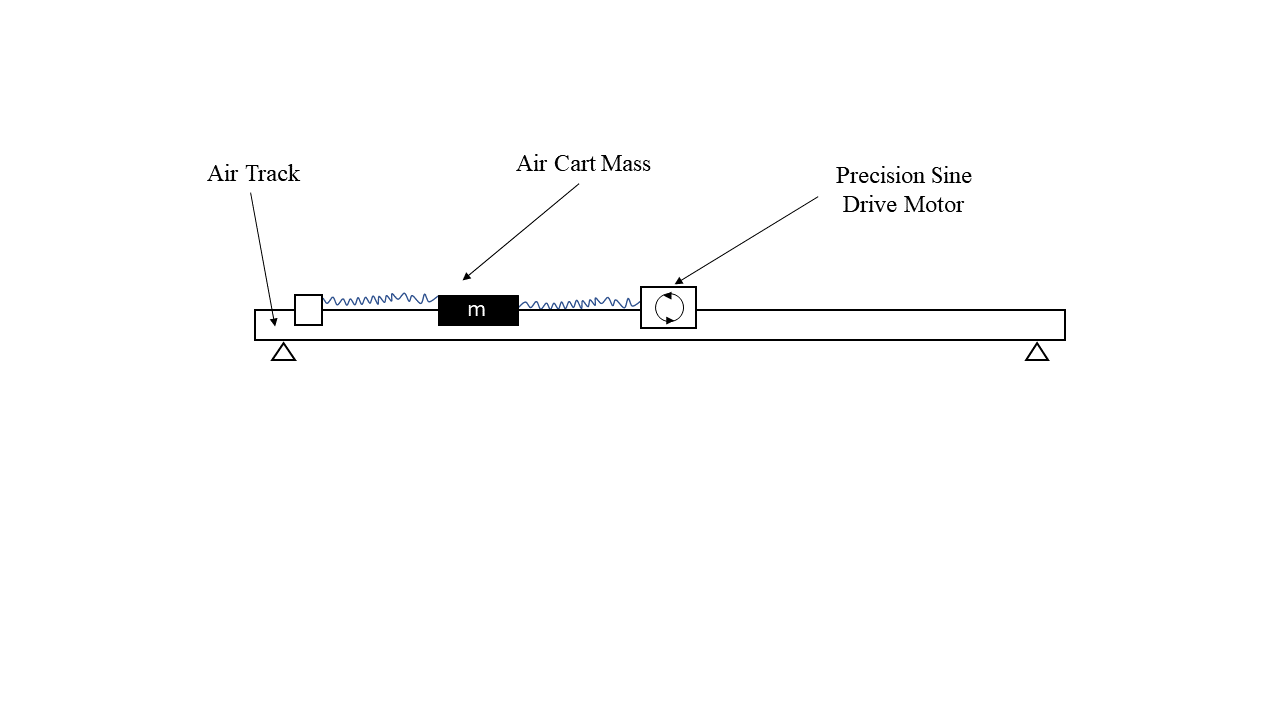
\includegraphics{AirTrack1Mass}
\caption{Air track configuration for one mass driven by a precision sine drive.}
\label{figure:AirTrack1Mass}
\end{figure}

\par To measure the resonance frequency, we first need to use the equation for forced, damped harmonic oscillation and solve for the theoretical natural resonance frequency. The force being applied to our system by the motor is

\begin{equation}
\textbf{F}_{driving} = F_0 cos(\omega t + \phi)
\label{eq:MotorForce}
\end{equation}

where $F_0$ is maximum force applied from the motor,$\omega$ is the varied frequency of the motor rotation, $t$ is time, and $\phi$ is an arbitrary phase adjustment. This gives a differential equation of the system described by

\begin{equation}
\ddot{x} + \frac{b}{m}\dot{x} + \frac{k}{m}x = \frac{F_0}{m} cos(\omega t = \phi) ,
\label{eq:DiffEqFDHM}
\end{equation}

where $\ddot{x}$ is the acceleration, $b$ is the damping, $\dot{x}$ is the velocity, $k$ is the spring constant, and $x$ is the displacement. This equation can be derived from the  general solution for a forced, damped harmonic oscillator and using equation (\ref{MotorForce}) as our force being applied. Futher solving equation (\ref{DiffEqFDHM}) gives us the solution

\begin{equation}
x(t) = Ae^{- \gamma t} cos( \omega_1 t) + \frac{\frac{F_0}{m}}{(\omega_0 - \omega)^2 + 4 \gamma^2 \omega^2} cos(\omega t + \phi)
\label{eq:solution1cart}
\end{equation}

where $\omega_1$ is the natural frequency, $\gamma = \frac{b}{2m}$, and $\omega_0 = \sqrt{\frac{k}{m}}$. The first term in equation (\ref{eq:solution1cart}) goes to zero after a period of time and is denoted the "transient solution". The second term remains after this period of time and is called the "steady-state term". This term is at its greatest amplitude when $\omega = \omega_0$. When this occurs, the system has achieved its resonance frequency. This resonance frequency is what we determine throughout the experiment.

\par To measure the resonance frequency for one mass, we first nudge the air cart while the air track is on and measure the period of oscillation. This gives us the natural period and natural frequency. We then calculate the angular frequency from these values. Then using the precision sine drive motor, we varied the frequency of motor oscillations and plotted the measured cart displacements resulting from the oscillations and determine the experimental resonance frequency. This was done in increments of 0.1 rad/s, and once we were close to within 0.05 rad/s from our theoretical resonance frequency we incremented by 0.01 rad/s until we demonstrated resonance frequency.




